\documentclass[12pt]{article}\usepackage[]{graphicx}\usepackage[]{color}
%% maxwidth is the original width if it is less than linewidth
%% otherwise use linewidth (to make sure the graphics do not exceed the margin)
\makeatletter
\def\maxwidth{ %
  \ifdim\Gin@nat@width>\linewidth
    \linewidth
  \else
    \Gin@nat@width
  \fi
}
\makeatother

\definecolor{fgcolor}{rgb}{0.345, 0.345, 0.345}
\newcommand{\hlnum}[1]{\textcolor[rgb]{0.686,0.059,0.569}{#1}}%
\newcommand{\hlstr}[1]{\textcolor[rgb]{0.192,0.494,0.8}{#1}}%
\newcommand{\hlcom}[1]{\textcolor[rgb]{0.678,0.584,0.686}{\textit{#1}}}%
\newcommand{\hlopt}[1]{\textcolor[rgb]{0,0,0}{#1}}%
\newcommand{\hlstd}[1]{\textcolor[rgb]{0.345,0.345,0.345}{#1}}%
\newcommand{\hlkwa}[1]{\textcolor[rgb]{0.161,0.373,0.58}{\textbf{#1}}}%
\newcommand{\hlkwb}[1]{\textcolor[rgb]{0.69,0.353,0.396}{#1}}%
\newcommand{\hlkwc}[1]{\textcolor[rgb]{0.333,0.667,0.333}{#1}}%
\newcommand{\hlkwd}[1]{\textcolor[rgb]{0.737,0.353,0.396}{\textbf{#1}}}%
\let\hlipl\hlkwb

\usepackage{framed}
\makeatletter
\newenvironment{kframe}{%
 \def\at@end@of@kframe{}%
 \ifinner\ifhmode%
  \def\at@end@of@kframe{\end{minipage}}%
  \begin{minipage}{\columnwidth}%
 \fi\fi%
 \def\FrameCommand##1{\hskip\@totalleftmargin \hskip-\fboxsep
 \colorbox{shadecolor}{##1}\hskip-\fboxsep
     % There is no \\@totalrightmargin, so:
     \hskip-\linewidth \hskip-\@totalleftmargin \hskip\columnwidth}%
 \MakeFramed {\advance\hsize-\width
   \@totalleftmargin\z@ \linewidth\hsize
   \@setminipage}}%
 {\par\unskip\endMakeFramed%
 \at@end@of@kframe}
\makeatother

\definecolor{shadecolor}{rgb}{.97, .97, .97}
\definecolor{messagecolor}{rgb}{0, 0, 0}
\definecolor{warningcolor}{rgb}{1, 0, 1}
\definecolor{errorcolor}{rgb}{1, 0, 0}
\newenvironment{knitrout}{}{} % an empty environment to be redefined in TeX

\usepackage{alltt}
\usepackage{latexsym}
\usepackage{fullpage}
\usepackage{graphicx}
\usepackage{endnotes}
\usepackage{setspace}
\usepackage{amsfonts}
\usepackage{caption}
\usepackage[abbr]{harvard}
\usepackage{multirow}
\usepackage{longtable}
%\usepackage{times}
\usepackage{lscape}
\usepackage{float}
\usepackage{mathpazo}

\usepackage{color}
%\usepackage{natbib}
%\usepackage[colorlinks=true,linkcolor=blue, citecolor=blue]{hyperref}

\usepackage{titlesec}
\titleformat*{\section}{\large\bfseries}
\titleformat*{\subsection}{\large\itshape}
\titleformat*{\subsubsection}{\large\itshape}
\titleformat*{\paragraph}{\large\itshape}
\titleformat*{\subparagraph}{\large\itshape}


\clubpenalty=9999 \widowpenalty=9999
\parskip=5.75pt


%-------------------------------------------------------
\IfFileExists{upquote.sty}{\usepackage{upquote}}{}
\begin{document}

\title{\textbf{Veto Player and Fiscal Policy Stability \footnote{Replication files are available on the author's Github account (http://github.com/haowang666)}}}
%\date{}
\bigskip
\onehalfspacing\author{
	Hao Wang \\ Department of Political Science\\Arizona State University\\haowang@asu.edu
	}
\maketitle \thispagestyle{empty}




\noindent \textbf{Keywords:} {veto player, public policy}

\bigskip

\noindent \textbf{Abstract:} {Veto player theory \cite{Tsebelis2002} predicts that the number of veto players influencing policy stability. While studies in OECD countries have shown supportive evidence \cite{TsebelisChang2004}, there is few work on policy stability in nondemocracies. This project uses a new data-set from GSRE (Global State Revenues and Expenditures data-set) and perform an empirical test on veto player and budget stability in authoritarian countries. Preliminary analysis show that even in authoritarian countries, institutional constraints (veto players) lead to incremental budget changes.}
\newpage

\doublespacing


\section{Introduction}
Veto player theory \cite{Tsebelis2002} defines 'veto players' as individuals or institutions whose agreement is required for a change of the status quo. This theory predicts that: when the number of veto players increase, the winning set that can defeat status quo will shrink, which in turn leads to higher policy stability. Since veto player is ultimately related to the level of institutional constraints, a corollary is that institutional checks leads to more stable, incremental policy outcomes. With many checks and balances in the government, it will be harder to move policies from status quo equilibrium. 

Tsebelis and Chang (2004) apply veto player theory in the budget changes of the 19 OECD countries. In their analysis, parties with more polarized positions are modeled as potential veto players who could have blocked the policy proposals. Their results show that countries with more veto players have more stable budget policies. 

On the other hand, veto player theory also implies that more veto players make politicians harder to adjust current policies. This is particularly salient in countries with multiple veto players (e.g. the United States). During some time periods with exogenous shocks, the policy stability can be harmful and politicians may react to the long-time stability with rapid changes of policies, which forms a policy punctuation. 


Punctuated Equilibrium Theory (PET) (John and Bevan 2012, Jones and Baumgartner 2012) argues that government budget shifts over and under attention to certain policy areas lead to long periods of stability and short periods of radical changes. Most empirical evidence, however, is drawn from developed democracies. Following Baumgartner et al. (2015) and Lam and Chan (2015), we explore the determinants of policy stability in different authoritarian regimes. We extend the existing theory by examining the variations among authoritarian countries. Our results suggest that institutionalization in the policy making process is an important factor that explains cross national variation.


\nocite{JohBevan2012} \nocite{JonesBaumgartner2012}
\nocite{TsebelisChang2004}
\nocite{LamChan2015}
\nocite{TsebelisChang2004}


\section{Argument} 

\subsection{Institutional Constraints}

Veto player $\Rightarrow$ unable to change policy rapidly $\Rightarrow$ long term incremental changes and short-term rapid changes $\Rightarrow$ punctual equilibrium \cite{DerekBaumgartner2016}. 








\subsection{Policy Punctuation}





\section{Data}
Data in this project comes from various sources. The dependent variable comes from the GSRE project (Global State Revenues and Expenditures dataset). GSRE is a comprehensive budget dataset based on the previous released historical documents from the International Monetary Fund (IMF). Comparing with the IMF COFOG dataset, GSRE increases coverage and accuracy of budgeting data for most authoritarian regimes and some democratic regimes. Since GSRE is built on IMF historical documents, it covers all independent states that have been or are the members of the IMF and are being coded as an authoritarian regime in the \cite{Geddesetal2014} dataset. 

Data on deliberative democracies and other regime-related variables come from the Varieties of Democracy (Vdem) project (Coppedge et al. 2016). Unlike the widely used democracy index like Polity \cite{Polity2015}, Vdem provides multidimensional measurements of regimes, including both democracies and autocracies. 

\nocite{Vdem2016}



Data on institutional constraints come from the political constraints index \cite{Henisz2000}. Henisz develops a measure of institutional commitment that is objective, extensive, and based in positive political theory. He uses a quantitative model to capture the competitiveness portion of the definition of democracy (competitiveness and participation) with a proxy of number of independent veto points over policy outcomes and distribution of preferences of those actors. The measure is objective, with clear rules for measurement and aggregation, however it incorporates some of the Polity data coding for <U+9225><U+6E0B>ndependent judiciary<U+9225><U+FFFD> that gives it a slight subjective bias. POLCON is based on strong assumptions about each actor<U+9225><U+6A9A> veto power. The measures are strongly correlated with the ICRG indexes and the Polity <U+9225><U+6DD3>xecutive Constraint<U+9225><U+FFFD> index. <U+9225><U+6DED>he new release of the political constraint dataset expands the scope of coverage to as many as 234 countries over the period 1800<U+9225><U+FFFD>2001. It also corrects a small number of computational, coding and factual errors in the previous release. The new database also includes country codes from the Cross-national time series data archive, Polity and the World Bank to facilitate matching this dataset to other international datasets that you may have. Finally, it contains the component variables used to construct the political constraint indexes.<U+9225><U+FFFD>




Data on decentralization draws from the Political Institution Index \cite{Becketal2001}. 

\nocite{KeeferStasavage2003}










\subsection{Measuring Dependent Variables}

I measure the budget volatility  as the simple euclidean distance of the between-year percentage shifts. It can be written in the following equation \ref{dv1}: $S_{jt}$ is the stability index of the country $j$ at a certain year $t$. Since government budget has various categories: $p_{it}$ denotes the percentage of $i$th category of total expenditure. $S_t$ will increase as the difference between $p_{it}$ and $p_{it-1}$ increases.

\begin{equation}
S_t = \sqrt{\sum_{i = 1}^i (p_{it} -p_{it-1})^2} 

\label{dv1}
\end{equation}








\subsection{Independent Variables}


\section{Results}


\subsection{Pooled OLS with Panel Corrected Standard Errors}




\subsection{Fixed Effect Panel Data}


\begin{table}[!htbp] \centering 
  \caption{Fixed Effect Model} 
  \label{fe} 
\begin{tabular}{@{\extracolsep{5pt}}lcccc} 
\\[-1.8ex]\hline 
\hline \\[-1.8ex] 
 & \multicolumn{4}{c}{\textit{Dependent variable:}} \\ 
\cline{2-5} 
\\[-1.8ex] & stability\_0 & stability\_1 & stability\_2 & stability\_3 \\ 
\\[-1.8ex] & (1) & (2) & (3) & (4)\\ 
\hline \\[-1.8ex] 
 v2x\_delibdem & 0.002 & 0.028 & $-$0.013 & $-$0.041 \\ 
  & (0.037) & (0.044) & (0.042) & (0.044) \\ 
  & & & & \\ 
 e\_h\_polcon5 & $-$0.024 & $-$0.042$^{*}$ & $-$0.037$^{*}$ & $-$0.003 \\ 
  & (0.019) & (0.022) & (0.021) & (0.022) \\ 
  & & & & \\ 
 e\_autoc & $-$0.002 & $-$0.005$^{**}$ & $-$0.002 & $-$0.002 \\ 
  & (0.002) & (0.002) & (0.002) & (0.002) \\ 
  & & & & \\ 
 v2mecenefm & 0.013$^{**}$ & $-$0.003 & 0.012$^{*}$ & 0.009 \\ 
  & (0.006) & (0.007) & (0.006) & (0.007) \\ 
  & & & & \\ 
 e\_peaveduc & $-$0.011$^{***}$ & $-$0.008$^{*}$ & $-$0.004 & $-$0.008$^{*}$ \\ 
  & (0.004) & (0.005) & (0.004) & (0.005) \\ 
  & & & & \\ 
 e\_migdppcln & 0.035$^{***}$ & 0.030$^{*}$ & 0.019 & 0.036$^{**}$ \\ 
  & (0.013) & (0.015) & (0.015) & (0.015) \\ 
  & & & & \\ 
 e\_migdpgro & 0.0002 & 0.0001 & $-$0.001 & 0.0002 \\ 
  & (0.0005) & (0.001) & (0.001) & (0.001) \\ 
  & & & & \\ 
 e\_peginiwi & 0.0001 & $-$0.001 & $-$0.001 & $-$0.0005 \\ 
  & (0.0005) & (0.001) & (0.001) & (0.001) \\ 
  & & & & \\ 
 e\_Civil\_War & $-$0.005 & $-$0.013 & $-$0.006 & $-$0.001 \\ 
  & (0.011) & (0.013) & (0.013) & (0.013) \\ 
  & & & & \\ 
 v2x\_corr & $-$0.008 & $-$0.105$^{***}$ & $-$0.067$^{*}$ & $-$0.098$^{**}$ \\ 
  & (0.034) & (0.040) & (0.039) & (0.041) \\ 
  & & & & \\ 
\hline \\[-1.8ex] 
Observations & 2,904 & 2,904 & 2,904 & 2,904 \\ 
R$^{2}$ & 0.011 & 0.008 & 0.007 & 0.007 \\ 
Adjusted R$^{2}$ & $-$0.031 & $-$0.034 & $-$0.035 & $-$0.035 \\ 
F Statistic (df = 10; 2784) & 3.141$^{***}$ & 2.367$^{***}$ & 2.076$^{**}$ & 2.024$^{**}$ \\ 
\hline 
\hline \\[-1.8ex] 
\textit{Note:}  & \multicolumn{4}{r}{$^{*}$p$<$0.1; $^{**}$p$<$0.05; $^{***}$p$<$0.01} \\ 
\end{tabular} 
\end{table} 




\subsection{Fiexed Effect with Two Way Effects}


\subsection{OLS with L-Kurtosis}


\begin{table}[!htbp] \centering 
  \caption{OLS Regression with L-Kurtosis as DV} 
  \label{lkols} 
\begin{tabular}{@{\extracolsep{5pt}}lcccc} 
\\[-1.8ex]\hline 
\hline \\[-1.8ex] 
 & \multicolumn{4}{c}{\textit{Dependent variable:}} \\ 
\cline{2-5} 
\\[-1.8ex] & y\_lk0 & y\_lk1 & y\_lk2 & y\_lk3 \\ 
\\[-1.8ex] & (1) & (2) & (3) & (4)\\ 
\hline \\[-1.8ex] 
 v2x\_delibdem & 0.038 & 0.126 & 0.087 & 0.078 \\ 
  & (0.073) & (0.142) & (0.147) & (0.140) \\ 
  & & & & \\ 
 e\_h\_polcon5 & 0.011 & $-$0.002 & 0.036 & $-$0.007 \\ 
  & (0.046) & (0.089) & (0.092) & (0.088) \\ 
  & & & & \\ 
 e\_autoc & 0.006 & 0.005 & 0.007 & 0.005 \\ 
  & (0.004) & (0.008) & (0.008) & (0.008) \\ 
  & & & & \\ 
 v2mecenefm & 0.002 & 0.002 & 0.001 & 0.002 \\ 
  & (0.008) & (0.016) & (0.017) & (0.016) \\ 
  & & & & \\ 
 e\_peaveduc & 0.008$^{***}$ & 0.004 & 0.006 & 0.005 \\ 
  & (0.003) & (0.006) & (0.006) & (0.006) \\ 
  & & & & \\ 
 e\_migdppcln & $-$0.026$^{**}$ & $-$0.025 & $-$0.021 & $-$0.022 \\ 
  & (0.011) & (0.020) & (0.021) & (0.020) \\ 
  & & & & \\ 
 e\_migdpgro & 0.002 & 0.0002 & $-$0.002 & 0.001 \\ 
  & (0.003) & (0.006) & (0.007) & (0.006) \\ 
  & & & & \\ 
 e\_peginiwi & 0.0001 & $-$0.003$^{***}$ & $-$0.003$^{***}$ & $-$0.003$^{***}$ \\ 
  & (0.001) & (0.001) & (0.001) & (0.001) \\ 
  & & & & \\ 
 e\_Civil\_War & 0.049 & 0.061 & 0.048 & 0.058 \\ 
  & (0.036) & (0.069) & (0.072) & (0.069) \\ 
  & & & & \\ 
 v2x\_corr & 0.013 & $-$0.027 & $-$0.020 & $-$0.045 \\ 
  & (0.030) & (0.059) & (0.061) & (0.058) \\ 
  & & & & \\ 
 Constant & 0.205$^{***}$ & 0.487$^{***}$ & 0.460$^{***}$ & 0.484$^{***}$ \\ 
  & (0.078) & (0.151) & (0.156) & (0.149) \\ 
  & & & & \\ 
\hline \\[-1.8ex] 
Observations & 112 & 112 & 112 & 112 \\ 
R$^{2}$ & 0.115 & 0.136 & 0.137 & 0.144 \\ 
Adjusted R$^{2}$ & 0.027 & 0.050 & 0.052 & 0.059 \\ 
Residual Std. Error (df = 101) & 0.049 & 0.095 & 0.098 & 0.094 \\ 
F Statistic (df = 10; 101) & 1.308 & 1.589 & 1.606 & 1.693$^{*}$ \\ 
\hline 
\hline \\[-1.8ex] 
\textit{Note:}  & \multicolumn{4}{r}{$^{*}$p$<$0.1; $^{**}$p$<$0.05; $^{***}$p$<$0.01} \\ 
\end{tabular} 
\end{table} 







\newpage

\section{Appendix}



\subsection{Descriptive Statistics}

Here I provide summary statistics of the variables I used in this study

\subsubsection{summary statistics of deliberative democracy}





\begin{table}[!htbp] \centering 
  \caption{Deliberative Democracy Statistics} 
  \label{delib} 
\begin{tabular}{@{\extracolsep{5pt}}lccccc} 
\\[-1.8ex]\hline \\[-1.8ex] 
Statistic & \multicolumn{1}{c}{N} & \multicolumn{1}{c}{Mean} & \multicolumn{1}{c}{St. Dev.} & \multicolumn{1}{c}{Min} & \multicolumn{1}{c}{Max} \\ 
\hline \\[-1.8ex] 
Deliberative Democracy & 6,373 & 0.201 & 0.225 & 0.001 & 0.881 \\ 
Justification on Public Policy & 6,382 & $-$0.067 & 1.226 & $-$3.125 & 3.415 \\ 
Justification on Common Goods & 6,382 & 0.083 & 1.153 & $-$3.394 & 2.868 \\ 
Respect for Counterarguments & 6,382 & $-$0.526 & 1.297 & $-$3.257 & 2.726 \\ 
Range of Consultation & 6,382 & $-$0.194 & 1.267 & $-$3.211 & 3.713 \\ 
Range of Engagement & 6,382 & $-$0.266 & 1.311 & $-$3.244 & 3.159 \\ 
\hline \\[-1.8ex] 
\end{tabular} 
\end{table} 


\subsubsection{summary statistics on institutional constraints}


\begin{table}[!htbp] \centering 
  \caption{Institutional Constraints} 
  \label{const} 
\begin{tabular}{@{\extracolsep{5pt}}lccccc} 
\\[-1.8ex]\hline 
\hline \\[-1.8ex] 
Statistic & \multicolumn{1}{c}{N} & \multicolumn{1}{c}{Mean} & \multicolumn{1}{c}{St. Dev.} & \multicolumn{1}{c}{Min} & \multicolumn{1}{c}{Max} \\ 
\hline \\[-1.8ex] 
Judical Constraints & 6,382 & 0.450 & 0.269 & 0.006 & 0.979 \\ 
Legislative Constraints & 6,354 & 0.385 & 0.282 & 0.024 & 0.959 \\ 
Institutionalization of Party & 6,381 & 0.492 & 0.273 & 0.006 & 0.986 \\ 
Institutionalizaed Democracy & 5,904 & 2.874 & 3.609 & 0 & 10 \\ 
Institutionalizaed Autocracy & 5,904 & 4.403 & 3.517 & 0 & 10 \\ 
Political Constraints Index-3 & 5,296 & 0.222 & 0.290 & 0.000 & 0.890 \\ 
Political Constraints Index-5 & 6,079 & 0.147 & 0.196 & 0.000 & 0.688 \\ 
\hline \\[-1.8ex] 
\end{tabular} 
\end{table} 



\subsubsection{summary statistics on federalism}


\begin{table}[!htbp] \centering 
  \caption{Division of Power (centrl-regional) Index} 
  \label{fed} 
\begin{tabular}{@{\extracolsep{5pt}}lccccc} 
\\[-1.8ex]\hline 
\hline \\[-1.8ex] 
Statistic & \multicolumn{1}{c}{N} & \multicolumn{1}{c}{Mean} & \multicolumn{1}{c}{St. Dev.} & \multicolumn{1}{c}{Min} & \multicolumn{1}{c}{Max} \\ 
\hline \\[-1.8ex] 
Division of Power & 5,774 & 0.304 & 0.330 & 0.000 & 0.991 \\ 
Regional Government Power & 5,782 & $-$0.325 & 1.286 & $-$2.664 & 2.775 \\ 
Local Government Power & 5,852 & 0.013 & 1.249 & $-$2.733 & 2.326 \\ 
\hline \\[-1.8ex] 
\end{tabular} 
\end{table} 



\subsubsection{summary statistics on other control variables}


\begin{table}[!htbp] \centering 
  \caption{Other Control Variables} 
  \label{control} 
\begin{tabular}{@{\extracolsep{5pt}}lccccc} 
\\[-1.8ex]\hline 
\hline \\[-1.8ex] 
Statistic & \multicolumn{1}{c}{N} & \multicolumn{1}{c}{Mean} & \multicolumn{1}{c}{St. Dev.} & \multicolumn{1}{c}{Min} & \multicolumn{1}{c}{Max} \\ 
\hline \\[-1.8ex] 
Media Censorship & 6,382 & $-$0.311 & 1.434 & $-$3.036 & 3.316 \\ 
Education & 6,184 & 4.470 & 2.691 & 0.004 & 13.285 \\ 
GDP pp(logged) & 5,839 & 7.629 & 0.886 & 5.315 & 10.667 \\ 
GDP growth & 5,807 & 1.763 & 6.388 & $-$61.493 & 86.946 \\ 
Income Inequality & 4,137 & 42.720 & 10.359 & 15.000 & 73.900 \\ 
Civial War & 6,200 & 0.090 & 0.286 & 0 & 1 \\ 
Oil Production Per Capita & 6,164 & 347.425 & 2,506.486 & 0.000 & 78,588.800 \\ 
Corruption Index & 6,382 & 0.552 & 0.232 & 0.028 & 0.946 \\ 
\hline \\[-1.8ex] 
\end{tabular} 
\end{table} 




\subsubsection{dependent variable components}

In the following table I report the components of dependent variables. It is measured as the percentage expenditure of total expenditure. Two indicators are dropped out in the further analysis due to technical concerns. The variable `subpentrans` contains too few points, and the variable `pensions` must be dropped due to the convergence issue in multiple imputation. 




\begin{table}[!htbp] \centering 
  \caption{Components of Budget Stability Measurements} 
  \label{comp} 
\begin{tabular}{@{\extracolsep{5pt}}lccccc} 
\\[-1.8ex]\hline 
\hline \\[-1.8ex] 
Statistic & \multicolumn{1}{c}{N} & \multicolumn{1}{c}{Mean} & \multicolumn{1}{c}{St. Dev.} & \multicolumn{1}{c}{Min} & \multicolumn{1}{c}{Max} \\ 
\hline \\[-1.8ex] 
expend\_security\_EXP & 3,034 & 0.166 & 0.123 & 0.000 & 0.712 \\ 
expenddefence\_EXP & 2,418 & 0.143 & 0.119 & 0.00001 & 0.712 \\ 
exp\_public\_order\_EXP & 1,300 & 0.059 & 0.034 & 0.000 & 0.248 \\ 
wagessalaries\_EXP & 3,981 & 0.293 & 0.128 & 0.00000 & 0.859 \\ 
pensions\_EXP & 1,131 & 0.058 & 0.065 & 0.000 & 0.392 \\ 
total\_welfare\_EXP & 2,927 & 0.238 & 0.127 & 0.00003 & 0.920 \\ 
education\_EXP & 2,624 & 0.133 & 0.061 & 0.00002 & 0.388 \\ 
health\_EXP & 2,337 & 0.058 & 0.032 & 0.00001 & 0.212 \\ 
social\_protection\_EXP & 1,451 & 0.055 & 0.073 & 0.000 & 0.599 \\ 
housing\_EXP & 1,084 & 0.035 & 0.036 & 0.000 & 0.420 \\ 
owelfarespend\_EXP & 1,334 & 0.067 & 0.077 & 0.00000 & 0.510 \\ 
\hline \\[-1.8ex] 
\end{tabular} 
\end{table} 



\subsubsection{dependent variable statistics}



\begin{table}[!htbp] \centering 
  \caption{Dependent Variable Statistics} 
  \label{imp} 
\begin{tabular}{@{\extracolsep{5pt}}lccccc} 
\\[-1.8ex]\hline 
\hline \\[-1.8ex] 
Statistic & \multicolumn{1}{c}{N} & \multicolumn{1}{c}{Mean} & \multicolumn{1}{c}{St. Dev.} & \multicolumn{1}{c}{Min} & \multicolumn{1}{c}{Max} \\ 
\hline \\[-1.8ex] 
Original & 5,299 & 0.103 & 0.144 & 0.00000 & 1.110 \\ 
Imputation 1 & 5,299 & 0.249 & 0.176 & 0.00001 & 1.318 \\ 
Imputation 2 & 5,299 & 0.256 & 0.172 & 0.00001 & 1.085 \\ 
Imputation 3 & 5,299 & 0.245 & 0.171 & 0.00001 & 1.810 \\ 
Imputation 4 & 5,299 & 0.253 & 0.173 & 0.00001 & 1.121 \\ 
Imputation 5 & 5,299 & 0.249 & 0.169 & 0.00001 & 1.064 \\ 
\hline \\[-1.8ex] 
\end{tabular} 
\end{table} 


Table \ref{imp} is 

\subsection{Missing Cases}

GSRE contains lots of missing cases. To avoid losing statistical powers and potential bias due to list-wise deletion, this article employs multiple imputation of the GSRE part data. Results reported in the paper are from the first imputation. Appendix includes the rest 4 imputations. 

The total missing map is showing in the corresponding figure. In this table, the components represent the percentage expenditure of each sector in terms of total expenditure. 


\begin{figure}
\begin{knitrout}
\definecolor{shadecolor}{rgb}{0.969, 0.969, 0.969}\color{fgcolor}
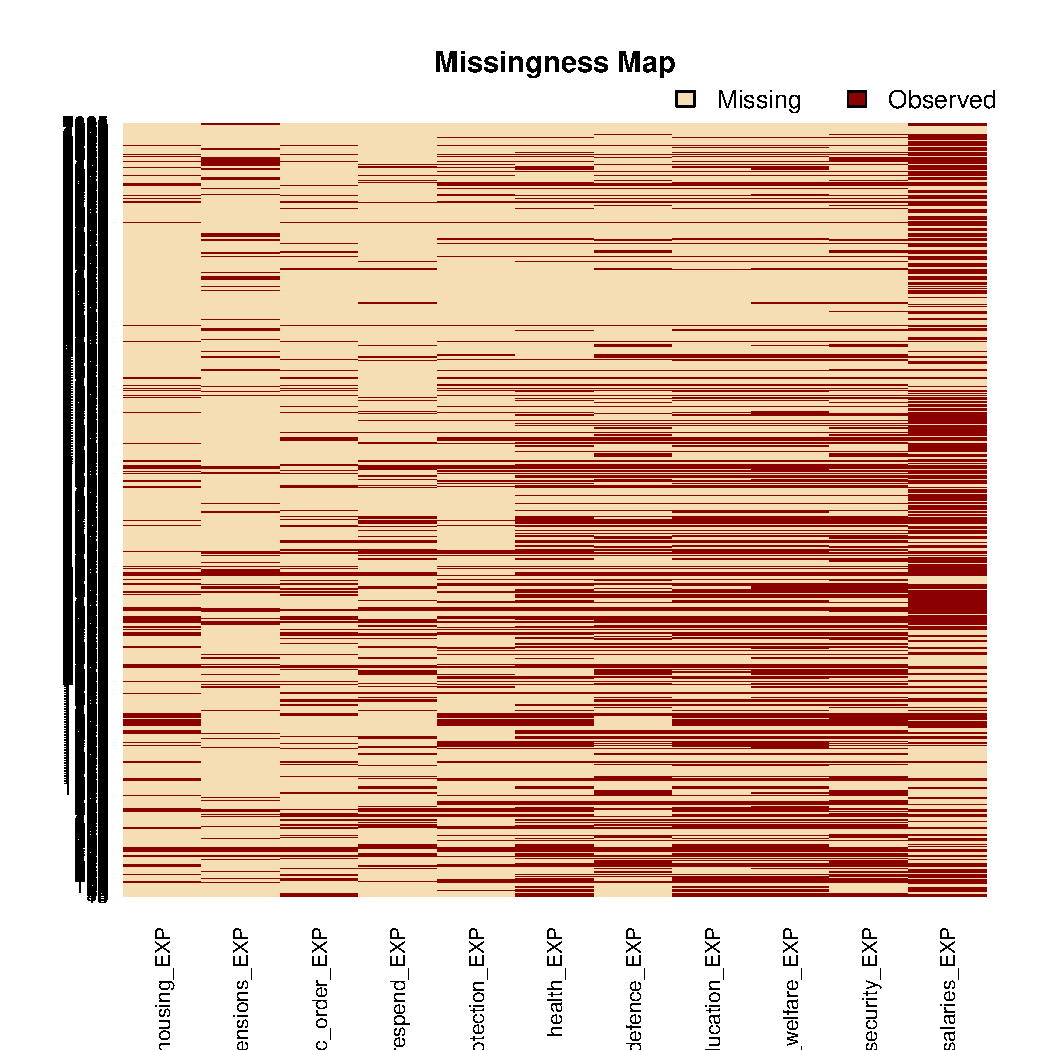
\includegraphics[width=\maxwidth]{figure/map-1} 

\end{knitrout}
\caption{Missingness Map of GSRE Data}
\label{figmiss}
\end{figure}


I also calculated results without multiple imputation: points that are missing in the GSRE database is set to be 0. Theoretically in this situation missing cases will contribute zero effects to the policy stability indicator. I calculate dependent variable while filling missing cases as 0. After the DV is imputed, I re-coded observations with 0 values as missing (This is because a completely missing case will yield 0 as the outcome). 




The density plot of stability index without imputation is shown in the following figure


\begin{figure}
\begin{knitrout}
\definecolor{shadecolor}{rgb}{0.969, 0.969, 0.969}\color{fgcolor}
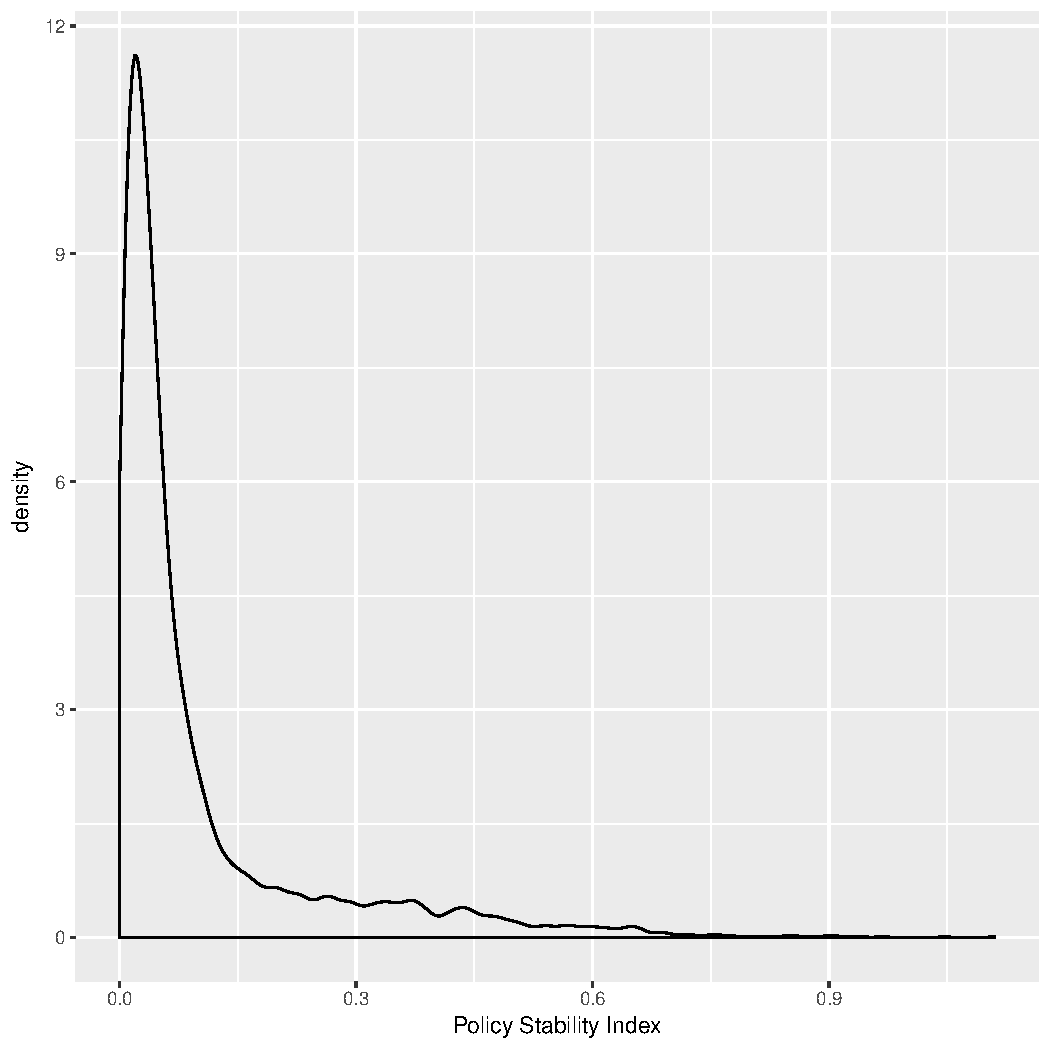
\includegraphics[width=\maxwidth]{figure/density-1} 

\end{knitrout}
\label{density}
\caption{Density Plot of Volatility Index}
\end{figure}


The relationship between the raw DV and the imputed DV is shown in the following graph. Due to the page limits only the relationships between the original dependent variable and the first two imputed dependent variables are displayed here. 







\newpage
\singlespacing 
\bibliography{Haowang.bib}
\bibliographystyle{apsr}


\end{document}
